\chapter{Simboličko izračunavanje}
\label{sec:Symbolics}

Današnji softver je veoma komplikovan i često funkcioniše na različitim nivoima arhitekture velikih projekata. Stoga je proces verifikacije softvera danas veoma značajan i delikatan. U procesu verifikacije se najčešće koriste ručno pisani testovi i pregledi koda od strane drugih programera. Uprkos svim ovim merama, greške su i dalje nezaobilazne --- jedan test može proveriti ponašanje koda za samo jedan ulaz. S obzirom da je nemoguće testirati sve ulaze zbog njihovog ogromnog broja (ukoliko posmatramo samo funkciju jedne promenljive koja prima 32-bitni ceo broj, broj mogućih ulaza je $2^{32}$) potrebno je da testovi dobro \emph{generalizuju} --- da pokrivaju opšte ali i neke specijalne ulaze. To se postiže uočavanjem da se vrednosti ulaza mogu razvrstati u klase po tome kakav izlaz uzrokuju. Ukoliko imamo funkciju koja deli dva broja, te klase mogu biti celi brojevi, realni brojevi, neke specijalne vrednosti specifične za operaciju deljenja (recimo $0$), kao i granice za tip podataka iz čijeg domena argumenti funkcije mogu uzeti vrednost. Čak i ovakav pristup, iako drastično smanjuje broj testova i eliminiše redundantne testove, i dalje zahteva relativno veliki broj testova u slučaju većih projekata i stoga je teško pronaći sve greške, pogotovo u slučajevima koji se retko dešavaju i ako ispoljavanje istih zavisi od stanja drugih komponenti ili pak nekih nedeterminističkih ponašanja samog sistema. Poželjno je čitav izvorni k\^od pokriti  testovima (engl. \emph{code coverage}) --- iako dostignuta pokrivenost koda od 100\% i dalje ne znači da taj k\^od ispravno radi.

\emph{Statička analiza koda} predstavlja analizu izvornog koda bez pokretanja istog sa ciljem ispitivanja stanja u kojima se može naći program i proveru rada jedinice koja se testira za mnogobrojne ulaze. Iako teorijski valjana, u praksi nailazi na puno problema --- osnovni je razlika u apstrakcijama koju prave statički analizator i programer, što otežava korišćenje ovakve analize u praksi.

\emph{Simboličko izvršavanje} \cite{SymbolicExecution} predstavlja sredinu između klasične verifikacije putem pisanja testova i statičke analize koda. Prilikom simboličkog izvršavanja, umesto stvarnih vrednosti ulaza koriste se \emph{simboličke promenljive}. Simbolička promenljiva nije vezana za specifičnu vrednost i analiza se dalje vrši samo nad njom --- samim tim se istovremeno mogu testirati višestruke klase sličnih ulaza. 

Primer simboličkog izvršavanja će biti opisan na isečku C koda sa slike \ref{fig:SymbolicExecCode}. Pretpostavimo da imamo deklarisanje promenljive \texttt{a}, \texttt{b} i \texttt{c} i da se neke operacije izvršavaju nad njima, reprezentovano komentarom u liniji $3$. U nekom trenutku se vrednosti tih promenljivih koriste kao uslovi od kojih zavisi prolaznost testa u poslednjoj liniji. Dodelimo svakoj promenljivoj simboličku vrednost --- \texttt{a = }$\alpha$, \texttt{b = }$\beta$, \texttt{c = }$\gamma$. Možemo izgraditi stablo izvršavanja i uslove koji moraju da važe nad simboličkim vrednostima $\alpha$, $\beta$ i $\gamma$ kako bi test u poslednjoj liniji prošao.

\begin{figure}[h!]
\begin{lstlisting}[language={}]
int a, b, c;

// ...

int x = 0, y = 0, z = 0;
if (a)      
    x = -2;
if (b < 5)  {
    if (!a && c)    
        y = 1;
    z = 2;
}

assert(x + y + z != 3);
\end{lstlisting}
\caption{Isečak C koda dat kao primer nad kojim će se prikazati simboličko izvršavanje.}
\label{fig:SymbolicExecCode}
\end{figure}

Ukoliko put izvršavanja programa zavisi od simboličke promenljive, kao što je to slučaj za izvorni k\^od sa slike \ref{fig:SymbolicExecCode}, simbolička promenljiva se konceptualno "grana" i analiza se nastavlja za oba slučaja posebno. Tako se dobija drvo izvršavanja, gde svaki put odgovara mnogim individualnim testovima koji bi uzrokovali prolazak izvršavanja tim putem. Vrednosti promenljivih u tim testovima moraju zadovoljiti uslove na kraju svakog puta --- tzv. \emph{uslove puta} (engl. \emph{path conditions}). Odgovarajuće stablo izvršavanja za izvorni k\^od sa slike \ref{fig:SymbolicExecCode} sa definisanim simboličkim vrednostima $\alpha$, $\beta$ i $\gamma$ se može videti na slici \ref{fig:SymbolicExecTree}. Svaka naredba dodele je uokvirena pravougaonikom dok je uslov uokviren elipsom. Boje grana odgovaraju istinitosnoj vrednosti uslova iz poslednje linije u tom trenutku. Na kraju svake grane se nalazi uslov puta za tu granu koje u nekim slučajevima može jedinstveno odrediti vrednost simboličke promenljive koja dovodi do prolaska tim putem ili u opštem slučaju generisati test primer koji dovodi do prolaska tim putem. Dakle, ukoliko je stablo simboličkog izvršavanja poznato, moguće je trivijalno generisati kontra-primere koji dokazuju da program ne radi kao što je očekivano.

\begin{figure}[h!]
\centering
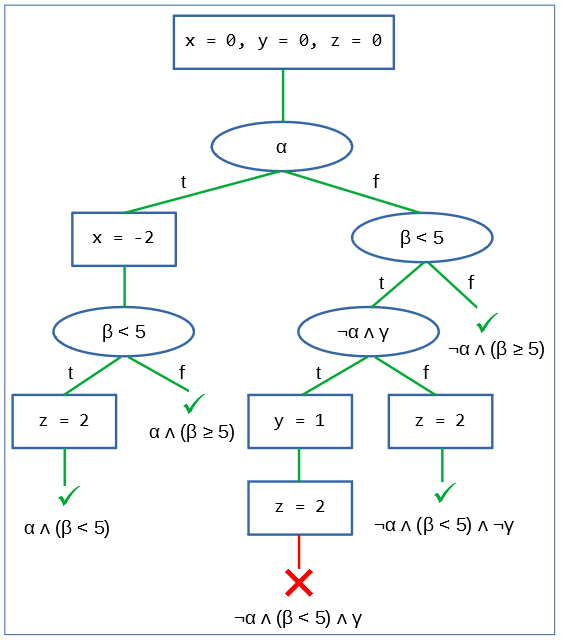
\includegraphics[scale=0.7]{images/sym_tree.png}
\caption{Drvo simboličkog izvršavanja na kom su prikazane sve putanje koje se razmatraju. Na kraju svake grane je napisan uslov koji mora da važi da bi se došlo do lista te grane.}
\label{fig:SymbolicExecTree}
\end{figure}

Simboličko izvršavanje, iako konceptualno moćno, ima par problema koji su uzrokovani pre svega kompleksnošću problema koji se rešava:
\begin{itemize}
    \item \emph{Eksplozija putanja} --- Broj puteva izvršavanja eksponencijalno zavisi od broja uslovnih grananja u kodu. Ukoliko imamo 3 naredbe grananja, broj puteva izvršavanja je $2^3=8$. Štaviše, petlje su još komplikovanije, jer ukoliko u petlji postoji uslov koji zavisi od simboličke vrednosti koja uzima vrednosti iz opsega 32-bitnog celog broja, broj puteva kroz petlju je u tom slučaju $2^{31}$, a u komplikovanijim slučajevima i beskonačan. Slično važi i za rekurziju.
    \item \emph{Ograničenja rešavača} --- Kako broj puteva raste, povećava se i broj uslova koji se moraju zadovoljiti prilikom nalaženja kontraprimera. Trivijalni algoritmi kao što su pretrage u dubinu i širinu nisu dovoljno efikasni. U nekim slučajevima je moguće osloniti se na \emph{SMT rešavače} \cite{SMT} za nalaženje kontra-primera kako bi se ublažio ovaj problem.
    \item \emph{Modelovanje podataka} (engl. \emph{heap modelling}) --- Kreiranje simboličkih struktura podataka i pokazivača nije jednostavan proces.
    \item \emph{Modelovanje okruženja} (engl. \emph{environment modelling}) --- Nije uvek jednostavno adaptirati mehanizam za česte potrebe prilikom dizajna softvera kao što je korišćenje eksternih biblioteka i sistemskih poziva ali i specifičnosti sistema.
\end{itemize}

Postoji dosta alata i biblioteka koje pružaju interfejs za simboličko izračunavanje u raznim programskim jezicima --- jedan od najpoznatijih alata za simboličko izračunavanje je \emph{KLEE} \cite{KLEE}, izgrađen nad \emph{LLVM} infrastruktorom \cite{LLVM} i dizajniran za analizu koda pisanog u programskom jeziku C. U ovom radu će simboličko izvršavanje biti korišćeno za detekciju razlika u vrednostima promenljivih uz pomoć biblioteka za programski jezik C\#.
